\documentclass[3p,times,procedia]{elsarticle}
\flushbottom

\usepackage{ecrc}
\usepackage[bookmarks=false]{hyperref}
    \hypersetup{colorlinks,
      linkcolor=blue,
      citecolor=blue,
      urlcolor=blue}

\volume{00}
\firstpage{1}
\journalname{Procedia Computer Science}
\runauth{C. Scherb et al.}
\jid{procs}

\usepackage{amssymb}
\usepackage{amsmath}
\usepackage{listings}
\usepackage{xcolor}
\usepackage{booktabs}
\usepackage{tikz}
\usetikzlibrary{positioning,arrows.meta,shapes.geometric,fit,backgrounds,calc}
\usepackage{tabularx}
\usepackage[figuresright]{rotating}

% tolerate long underscore-heavy texttt identifiers
\sloppy
\emergencystretch=3em
\hfuzz=2pt
\vfuzz=2pt

\lstdefinestyle{jsoncode}{
  basicstyle=\ttfamily\footnotesize,
  numbers=none,
  tabsize=2,
  columns=fullflexible,
  breaklines=true
}

\begin{document}
\begin{frontmatter}

\dochead{30th International Conference on Knowledge-Based and Intelligent Information \& Engineering Systems (KES 2026)}

\title{Closing the Triage Loop: MCP-mediated KLEE Validation of LLM-Reported C/C++ Vulnerabilities}

\author[a]{Christopher Scherb\corref{cor1}}
\author[a]{Alexander Trapp}
\author[a]{Ruben Hutter}
\author[a]{Nico Bachmann}
\author[a]{Luc Bryan Heitz}

\address[a]{University of Applied Sciences and Arts Northwestern Switzerland, Bahnhofstrasse 6, 5210 Windisch, Switzerland}

\begin{abstract}
Large language models are proficient at flagging plausible vulnerability candidates in C/C++ code but cannot produce concrete proofs of exploitability. Symbolic execution engines like KLEE produce concrete crashing inputs but need a harness and the right preconditions. We close this loop with \textsc{klee-mcp}: a stateless Model Context Protocol (MCP) server that exposes KLEE as five tools (\texttt{auto\_harness}, \texttt{verify\_vulnerability}, \texttt{check\_reachability}, \texttt{emit\_reproducer}, \texttt{generate\_harness}) to an LLM auditor, plus a Claude Code skill that drives the end-to-end workflow from a single natural-language instruction. The auditor emits structured candidates (CWE, tainted inputs, semantic bounds); the server auto-builds a KLEE harness, optionally links whole-library LLVM bitcode, either confirms the bug with a byte-accurate concrete input or proves it infeasible under the supplied bounds, and emits a disclosure-ready standalone reproducer (\texttt{reproduce.c} plus \texttt{poc.bin}) together with an exploitability classification and heuristic CVSS-3.1 vector. On 14 candidates spanning toy CWE programs and libpng 1.6.47 (full library linked as a 2.2\,MB bitcode) the pipeline agrees with ground truth in 14/14 cases, and surfaces an unchecked precondition in \texttt{png\_format\_number} (\texttt{pngerror.c:140}) for which KLEE synthesises a concrete one-byte out-of-bounds write trigger in 4.2\,s. All libpng-internal callers respect the function's contract, so this is a defense-in-depth finding rather than a remotely-reachable CVE. We additionally reproduce CVE-2015-8540 in \texttt{png\_check\_keyword}: KLEE synthesises a concrete crashing input in 1.26\,s, the same out-of-bounds read is still reachable in libpng~1.6.47, and a counterfactual LLM bound that models the caller-side fix flips the verdict to infeasible. We argue that LLM-supplied semantic bounds encode the caller contract under which safety is being verified, not a performance knob, and demonstrate a self-correcting auto-relax retry when those bounds are wrong.
\end{abstract}

\begin{keyword}
Vulnerability triage \sep symbolic execution \sep KLEE \sep large language models \sep Model Context Protocol \sep coordinated disclosure
\end{keyword}
\cortext[cor1]{Corresponding author. Email: christopher.scherb@fhnw.ch}
\end{frontmatter}

\section{Introduction}
\label{sec:intro}

Triage is the bottleneck of C/C++ vulnerability work: static analysers emit thousands of candidates, most of which are false positives, and language models are good at proposing plausible candidates but cannot produce concrete crashing inputs. Symbolic execution --- KLEE \cite{klee} being the standard reference --- can produce such inputs if given a harness with the right preconditions. We join these two halves through the Model Context Protocol (MCP) \cite{mcp}: KLEE is exposed as an MCP server, and a tool-using LLM agent (Claude Code) commits to a structured candidate schema that the server turns into a harness and a verdict. The loop runs from a single natural-language instruction and closes with either a byte-accurate crashing input or a proof of infeasibility under the LLM's declared preconditions.

\paragraph{Contributions.} \textbf{\textsc{klee-mcp}}\footnote{Source, skill, and reproducible benchmark: \url{https://github.com/FHNW-Security-Lab/klee-mcp}} is a stateless MCP server exposing KLEE as five tools, plus a Claude Code skill that drives the full triage pipeline. Its \emph{candidate schema} (CWE, tainted inputs, LLM-supplied semantic bounds, retry policy) turns LLM bounds into \texttt{klee\_assume} predicates that the server can \emph{automatically relax} on an infeasible verdict --- surfacing, rather than hiding, cases where the LLM's precondition was wrong. For every confirmed bug the server emits a standalone \texttt{reproduce.c}, a \texttt{poc.bin}, and an exploitability classification (primitive, severity, region, CVSS-3.1 vector) aimed at a coordinated-disclosure workflow. As a proof-of-concept evaluation we run 14 candidates spanning toy CWE programs, bounded/unbounded sensitivity pairs, and libpng~1.6.47 as a whole-library 2.2\,MB LLVM bitcode; 14/14 verdicts agree with ground truth. We further reproduce the CVE-2015-8540 pattern in \texttt{png\_check\_keyword}, confirming the same OOB in libpng 1.6.19 and 1.6.47 from the concrete byte-level trigger KLEE synthesises.

\section{Design}
\label{sec:design}

Figure~\ref{fig:pipeline} shows the pipeline. The LLM auditor (Section~\ref{sec:skill}) emits candidate JSON objects conforming to the candidate schema (Listing~\ref{lst:candidate}). Each candidate flows through the MCP server's tools (Section~\ref{sec:tools}) and produces a structured verdict plus, for confirmed candidates, a reproducer and an exploitability classification.

\begin{figure}[t]
\centering
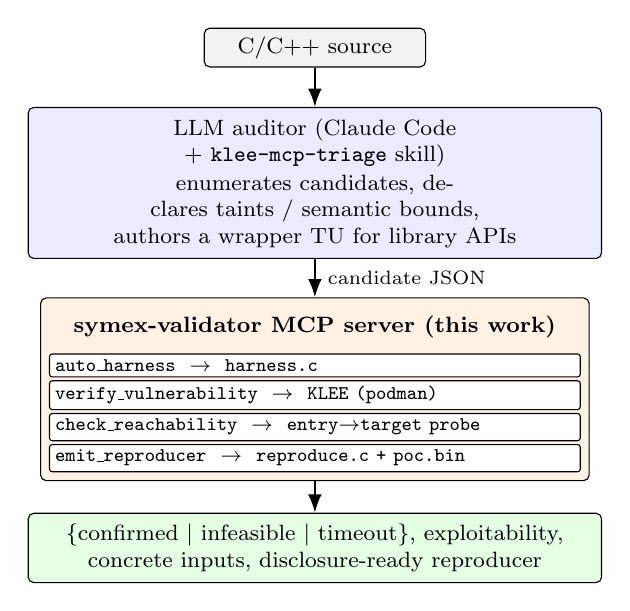
\begin{tikzpicture}[
  font=\footnotesize,
  box/.style={draw, rounded corners=2pt, align=center, inner sep=4pt,
              text width=70mm},
  src/.style ={draw, rounded corners=2pt, align=center, inner sep=3pt,
               fill=gray!10, text width=26mm},
  tool/.style={draw, rounded corners=1pt, align=left, inner sep=2pt,
               fill=white, font=\scriptsize\ttfamily, text width=66mm},
  llm/.style ={box, fill=blue!8},
  result/.style ={box, fill=green!10},
  srvtitle/.style={font=\footnotesize\bfseries, align=center},
  arr/.style ={-Latex, thick},
  node distance=5mm,
]

\node[src] (src) {C/C++ source};

\node[llm, below=5mm of src] (llm) {%
  LLM auditor (Claude Code + \texttt{klee-mcp-triage} skill)\\[1pt]
  enumerates candidates, declares taints / semantic bounds,\\
  authors a wrapper TU for library APIs};

\node[srvtitle, below=6mm of llm] (srvtitle)
  {symex-validator MCP server (this work)};
\node[tool, below=2pt of srvtitle] (t1)
  {auto\_harness \ $\rightarrow$ \ harness.c};
\node[tool, below=1pt of t1] (t2)
  {verify\_vulnerability \ $\rightarrow$ \ KLEE (podman)};
\node[tool, below=1pt of t2] (t3)
  {check\_reachability \ $\rightarrow$ \ entry$\to$target probe};
\node[tool, below=1pt of t3] (t4)
  {emit\_reproducer \ $\rightarrow$ \ reproduce.c + poc.bin};

\begin{scope}[on background layer]
  \node[draw, rounded corners=2pt, fill=orange!10,
        inner sep=3pt, fit=(srvtitle)(t1)(t2)(t3)(t4)] (srv) {};
\end{scope}

\node[result, below=4mm of srv] (res) {%
  \{confirmed $\mid$ infeasible $\mid$ timeout\}, exploitability,\\
  concrete inputs, disclosure-ready reproducer};

\draw[arr] (src) -- (llm);
\draw[arr] (llm) -- node[right=1pt,font=\scriptsize] {candidate JSON} (srv.north);
\draw[arr] (srv) -- (res);

\end{tikzpicture}
\caption{\textsc{klee-mcp} pipeline. The LLM is the auditor; the MCP server is a stateless tool host around KLEE.}
\label{fig:pipeline}
\end{figure}

\subsection{Candidate schema}
\label{sec:schema}

A candidate is a JSON object committing the LLM to a precise claim. Listing~\ref{lst:candidate} shows an example. The mandatory fields are \texttt{source\_file}, \texttt{function\_name}, \texttt{cwe}. The remaining fields are optional refinements:

\begin{itemize}
    \item \texttt{tainted\_inputs} lists which parameters are attacker-controlled. If omitted, the server infers one symbolic taint per parameter from the function prototype.
    \item \texttt{assumptions} and \texttt{loop\_bounds} carry LLM-supplied semantic bounds. They are delivered to KLEE as \texttt{klee\_assume} calls and only applied when \texttt{use\_bounds=true}. Example: the LLM knows that a size field in a network packet never exceeds 1500, so it emits \texttt{loop\_bounds: \{len: 1500\}}.
    \item \texttt{auto\_relax\_on\_infeasible}: if the bounded run returns \texttt{infeasible}, the server transparently retries without bounds and returns the relaxed verdict, annotated with \texttt{initial\_verdict=infeasible} and a warning in the \texttt{notes}. This is what catches the case of \emph{wrong} LLM bounds.
    \item \texttt{extra\_bitcodes}: a list of pre-built LLVM \texttt{.bc} files that the runner \texttt{llvm-link}s onto the harness before KLEE. This enables whole-library targets (Section~\ref{sec:impl}).
\end{itemize}

\begin{lstlisting}[style=jsoncode, caption={Candidate JSON for the libpng \texttt{png\_format\_number} OOB write.}, label={lst:candidate}]
{"source_file": "examples/real/whole_lib_format_number.c",
 "function_name": "fuzz_format_number", "cwe": "CWE-787",
 "tainted_inputs": [
   {"name":"format",     "c_type":"int",          "size_bytes":4},
   {"name":"number",     "c_type":"size_t",       "size_bytes":8},
   {"name":"end_offset", "c_type":"unsigned int", "size_bytes":4}],
 "loop_bounds": {"end_offset":16, "number":256, "format":8},
 "use_bounds": true, "auto_relax_on_infeasible": true,
 "extra_bitcodes": ["realworld/bitcode/libpng.bc"],
 "timeout_s": 120, "max_memory_mb": 16000}
\end{lstlisting}

\subsection{MCP tools}
\label{sec:tools}

The server exposes five tools. \texttt{auto\_harness} (\emph{Phase 0}): given \texttt{source\_file + function\_name + cwe}, parse the function prototype, infer taints with sensible defaults (scalar / 256-byte buffer / NULL for \texttt{size\_bytes=0}), and return the generated harness plus the inferred taint list. \texttt{verify\_vulnerability} (\emph{Phase 1}) is the main entry: it accepts the full candidate and runs KLEE inside \texttt{docker.io/klee/klee:3.1} under rootless podman, returning a \texttt{verdict} $\in$ \{confirmed, infeasible, timeout, build\_failed, klee\_error\}, the concrete \texttt{.ktest} hex, per-symbolic-variable decoded values, and (when confirmed) an exploitability classification (Section~\ref{sec:exploit}). \texttt{check\_reachability\_tool} (\emph{Phase 2}) takes an \texttt{entry\_function} (an LLM-picked realistic API, not \texttt{main}) and a \texttt{target\_function}, patches a scratch copy of the source to insert \texttt{klee\_report\_error} at the target, drives the entry function symbolically, and reports whether KLEE reaches the probe. \texttt{emit\_reproducer} (\emph{Phase 3}) writes a standalone \texttt{reproduce.c} inlining the KLEE-synthesised concrete values, a \texttt{poc.bin} of the raw bytes, and a gcc+ASan run recipe. \texttt{generate\_harness\_tool} is a manual escape hatch returning a harness from an explicit taint spec when auto-inference is inadequate.

\subsection{Orchestrator skill}
\label{sec:skill}

The Claude Code skill \texttt{klee-mcp-triage} is triggered by natural-language instructions such as ``analyze \texttt{X} with klee-mcp''. It enumerates source files, runs candidate hunting with a pattern-driven prompt, and then invokes the MCP tools per candidate in the order Phase~0 $\rightarrow$ Phase~1 $\rightarrow$ Phase~2 $\rightarrow$ Phase~3. For library APIs that require state setup (libpng's \texttt{png\_create\_read\_struct}, libxml2's \texttt{xmlReadMemory}), the skill authors a small wrapper translation unit that exposes a simpler symbolic surface and forward-declares the library APIs it calls; the wrapper is linked against the library's whole-program bitcode at verify time via \texttt{extra\_bitcodes}. A concrete example is the libpng push-mode harness used in Section~\ref{sec:eval}: 50 lines of C that drives the full libpng push parser with 8 symbolic attacker bytes. The skill finally writes a single markdown report per run, with a summary table, per-confirmed-bug disclosure template (advisory header, root cause, reproduction, concrete inputs, suggested fix, coordinated-disclosure email boilerplate), rescued false positives, and unresolved candidates.

\section{Implementation}
\label{sec:impl}

KLEE \cite{klee} 3.1 and its runtimes (uClibc, POSIX) run inside a pinned container image with LLVM/clang 13, STP, and MiniSat; the server invokes it via rootless podman with \texttt{:Z} bind mounts, so no privileged operations are required on the host. Our function-level driving strategy is an instance of under-constrained symbolic execution \cite{ucklee}.

For each tainted input the harness generator emits either \texttt{klee\_make\_symbolic} on a scalar or on a declared buffer (typed by the caller-supplied \texttt{c\_type}, with a fallback for libpng-style typedef'd pointer types). LLM bounds are emitted as \texttt{klee\_assume} calls. A pointer taint with \texttt{size\_bytes=0} means ``pass NULL'' --- the idiom for exercising CWE-476 without symbolic pointer values.

For targets larger than a single translation unit, we ship \texttt{build\_lib\_bc.sh}: it compiles every \texttt{.c} in a source tree to \texttt{.bc} via clang in the KLEE container, then \texttt{llvm-link}s them. On libpng~1.6.47 plus zlib~1.3.1 this produces a 2.2\,MB combined bitcode in under one minute (30 TUs). The runner stages it alongside the harness before calling KLEE.

KLEE emits a \texttt{.err} file for \emph{every} discovered error, including side effects that are not memory-safety bugs (libpng's own \texttt{abort()}, KLEE's internal \texttt{model}/\texttt{external} warnings). We therefore map each CWE to the KLEE error classes that actually confirm the bug and filter out the rest, logging the ignored errors for transparency. The reachability tool patches a copy of the source to insert \texttt{klee\_report\_error} at the target, then runs KLEE with \texttt{--exit-on-error-type=ReportError} so the first reaching path aborts cleanly and the entry-function input becomes the reachability witness.

\section{Exploitability classification}
\label{sec:exploit}

A key deliverable for a coordinated-disclosure workflow is \emph{severity context}: is this crash an arbitrary write an attacker can weaponise, or is it a bounded denial-of-service? We add a heuristic classifier (Table~\ref{tab:prim}) that runs after every confirmed verdict. It consumes (i) the KLEE \texttt{.err} file's \texttt{Info:} section, (ii) the candidate's declared CWE, and (iii) the source line at the sink.

\begin{table}[t]
\caption{Exploitability primitives. The classifier combines KLEE's faulting-address expression (symbolic vs concrete) with the declared CWE and a source-line read/write heuristic to assign one of these labels to each confirmed verdict.}
\label{tab:prim}
\begin{tabular*}{\hsize}{@{\extracolsep{\fill}}lll@{}}
\toprule
\textbf{Primitive} & \textbf{Operation} & \textbf{Default severity} \\
\midrule
\texttt{arbitrary\_write}  & write, symbolic address  & CRITICAL \\
\texttt{bounded\_write}    & write, concrete address  & HIGH     \\
\texttt{arbitrary\_read}   & read, symbolic address   & HIGH     \\
\texttt{bounded\_read}     & read, concrete address   & MEDIUM   \\
\texttt{uaf\_read/write}   & read/write on freed obj  & HIGH     \\
\texttt{null\_deref}       & read at 0                & MEDIUM   \\
\texttt{double\_free}      & free of freed ptr        & HIGH     \\
\texttt{integer\_overflow} & arith, no direct mem eff & LOW      \\
\texttt{div\_by\_zero}     & arith                    & LOW      \\
\texttt{crash}             & abort/assert             & LOW      \\
\bottomrule
\end{tabular*}
\end{table}

The \emph{symbolic-address} flag is the key distinguishing signal. A KLEE \texttt{.err} \texttt{Info:} block contains an \texttt{address:} line; if the value is a K-Query expression (e.g., \texttt{(Add w64 X (ReadLSB w64 0 whereami))}), the attacker controls which address is dereferenced and the primitive is the \emph{arbitrary} variant. A concrete integer means KLEE resolved the address to a specific location, so the primitive is \emph{bounded}.

The classifier also extracts (i) the target memory region (\texttt{stack} / \texttt{heap} / \texttt{static}) from KLEE's allocation note (\texttt{MO... allocated at ...: \%x = alloca i32} vs \texttt{malloc}), with a CWE-driven fallback, and (ii) a \emph{program-counter-overwrite possibility} flag that is \texttt{true} for arbitrary writes and for stack-located bounded writes. A heuristic CVSS-3.1 base vector is attached for disclosure-template prefill (the paper uses these values verbatim in Section~\ref{sec:eval}; they should be refined per engagement context).

\section{Evaluation}
\label{sec:eval}

\subsection{Setup}

All runs use the same environment: Arch Linux host, rootless podman 5.8.2, \texttt{docker.io/klee/klee:3.1} (KLEE 3.1, LLVM/clang 13, STP + MiniSat). Each candidate is capped at 16\,GB RSS and a per-candidate wall-time budget (30--180\,s). A single command (\texttt{python benchmark/run\_bench.py}) runs all 14 candidates and writes \texttt{benchmark/results.csv}.

\subsection{Benchmark}

Table~\ref{tab:results} lists all 14 candidates. Ground-truth verdicts are encoded in each candidate JSON (\texttt{expected\_verdict}). The benchmark covers five phases: (1) toy programs exercising each target CWE, (2) LLM bounds + auto-relax, (3) reachability, (4) extracted real libpng functions (self-contained TU), and (5) whole-library libpng+zlib bitcode.

\begin{table}[t]
\caption{14-candidate benchmark. B\,=\,\texttt{use\_bounds=true}; R\,=\,server auto-relaxed after a bounded infeasible run. All verdicts match ground truth.}
\label{tab:results}
\scriptsize
\setlength{\tabcolsep}{3pt}
\begin{tabular*}{\hsize}{@{\extracolsep{\fill}}lccccrl@{}}
\toprule
\textbf{Candidate} & \textbf{CWE} & \textbf{Exp.} & \textbf{Verdict} & \textbf{B/R} & \textbf{Wall} & \textbf{Primitive / severity} \\
\midrule
\multicolumn{7}{@{}l}{\emph{Phase 1 --- toy examples}} \\
bof\_01                    & 121 & c. & c. & --         & 1.0\,s & bounded\_write / HIGH \\
intoverflow\_01            & 190 & c. & c. & --         & 2.4\,s & bounded\_write / HIGH \\
null\_01                   & 476 & c. & c. & --         & 0.9\,s & null\_deref / MED \\
uaf\_01                    & 416 & c. & c. & --         & 0.9\,s & uaf\_read / HIGH \\
safe\_01 (neg.)            & 121 & i. & i. & --         & 1.1\,s & --- \\
\midrule
\multicolumn{7}{@{}l}{\emph{Phase 2 --- LLM bounds \& auto-relax}} \\
bof\_01\_bounded           & 121 & c. & c. & B          & 0.9\,s & bounded\_write / HIGH \\
bof\_01\_tootight          & 121 & c. & c. & B\,R       & 0.9\,s & bounded\_write / HIGH \\
\midrule
\multicolumn{7}{@{}l}{\emph{Phase 3a --- extracted real libpng}} \\
libpng\_fp\_number         & 125 & i. & i. & B          & 30.9\,s & --- \\
libpng\_fp\_number\_bug    & 125 & c. & c. & B          & 5.9\,s & bounded\_read / MED \\
libpng\_fp\_number\_unb.   & 125 & c. & c. & --         & 9.4\,s & \textbf{arbitrary\_read} / HIGH \\
\midrule
\multicolumn{7}{@{}l}{\emph{Phase 3b --- whole-library libpng+zlib bitcode}} \\
libpng\_sig\_cmp           & 125 & i. & i. & B          & 5.1\,s & --- \\
libpng\_fp\_whole          & 125 & i. & i. & B          & 42.9\,s & --- \\
libpng\_push\_read         & OTH & i. & i. & B          & 4.1\,s & --- \\
libpng\_format\_number     & 787 & c. & c. & B          & 4.2\,s & arbitrary\_write$^\dagger$ \\
\bottomrule
\end{tabular*}
{\scriptsize $^\dagger$ Contract-violation finding, not internally reachable in libpng 1.6.47; see~\S\ref{sec:eval}.}
\end{table}

\paragraph{Result: 14/14 verdicts match ground truth.} Median wall time 2.4\,s; worst case 42.9\,s on the whole-library \texttt{png\_check\_fp\_number} exhaustion. Memory usage stayed well below the 16\,GB cap on every row. Phase-1 and -2 rows complete sub-second; extracted libpng targets (P3a) take 6--31\,s; whole-library linked targets (P3b) 4--43\,s.

\paragraph{Confirmed-vs-infeasible separation (C1).} Seven rows return \texttt{confirmed} with a byte-accurate KLEE-synthesised \texttt{.ktest}; the remaining seven return \texttt{infeasible} with KLEE's \texttt{done: completed paths = N, partially completed = 0} --- proofs under the declared bound. The sensitivity pair \texttt{libpng\_fp\_number} (bounded, infeasible in 30.9\,s, 1438 completed paths) vs \texttt{libpng\_fp\_number\_unb.} (unbounded, confirmed in 9.4\,s) shows both verdicts are correct under their respective contracts: the bounded run proves the loop safe \emph{given} a truthful \texttt{size}; the unbounded run shows the function trusts \texttt{size} blindly, so a caller over-reporting \texttt{size} causes an OOB read. Bounds therefore encode the \emph{precondition} under which safety is being verified, not a performance knob.

\paragraph{LLM bounds as caller contracts, self-correcting (C2).} Row \texttt{bof\_01\_tootight} injects a deliberate LLM error: \texttt{loop\_bounds=\{len: 10\}} for a bug that triggers at \texttt{len > 16}. The bounded run returns \texttt{infeasible}; the server auto-relaxes and returns \texttt{confirmed} in 0.9\,s with \texttt{initial\_verdict=infeasible}, \texttt{relaxed\_retry\_performed=true}, and a notes field ``\emph{LLM bounds ruled out the crashing input}'' --- the pipeline surfaces LLM mis-modelling rather than silently mis-verifying. On real-library targets the speedup is load-bearing: an unbounded run of the libpng FP state machine timed out at 60\,s with 1700 partial paths; with \texttt{loop\_bounds=\{size: 4\}} the same run exhausts 1438 complete paths in 30.9\,s.

\paragraph{Historical CVE reproduction: CVE-2015-8540 \cite{cve20158540}.} We extracted \texttt{png\_check\_keyword} from libpng~1.6.19 (last release before the 1.6.20 fix) into a byte-identical standalone TU, driven with a 4-byte symbolic non-null-terminated \texttt{key} and an 80-byte output buffer. KLEE \textbf{confirmed the OOB read at line~43 in 1.26\,s}, synthesising \texttt{key = 0x01\,0x01\,0x01\,0x01}: the \texttt{while (*key \&\& key\_len < 79)} loop reads \texttt{key[4]}, one byte past the allocation. Extracting the same function from libpng~1.6.47 (body preserved verbatim, moved to pngset.c) and running the identical harness yields \textbf{the same OOB at line~34 in 1.26\,s with the identical trigger}; the 1.6.20 fix lived in callers (null-terminating before invocation), not inside \texttt{png\_check\_keyword}. Adding the counterfactual LLM bound \texttt{key[3] == 0} (modelling the caller contract) flips the verdict to \textbf{infeasible in 1.17\,s after exhausting 103 completed paths}, directly illustrating on a real CVE that LLM bounds encode caller contracts and that the same function is safe-under-contract and unsafe-off-contract.

\paragraph{Cross-library audit.} A focused libpng tRNS chunk-handler harness (valid prefix, symbolic length and payload) timed out at 240\,s --- real handler exercised, no matching error. A libjpeg-turbo~3.0.4 harness (whole-library 3.5\,MB bitcode) through \texttt{jpeg\_read\_header} returned infeasible in 5.4\,s but only 1 completed path: KLEE~3.1 does not model the \texttt{longjmp}-based error paths, so the first malformed marker collapses exploration. A libxml2~2.12.6 harness (9.4\,MB bitcode, 106 TUs) calling \texttt{xmlReadMemory} on 32 symbolic bytes returned infeasible in 23\,s with \textbf{11 completed paths and 523\,K LLVM instructions executed} --- an end-to-end second-library result. Where the pipeline does not find a bug, the failure mode is an engine-side limit we can characterise.

\paragraph{Whole-library bitcode scales to real code (C3).} Rows 11--14 link against a single 2.2\,MB \texttt{libpng+zlib.bc} built once from 30 TUs. Row 13 (\texttt{libpng\_push\_read}) is the realistic fuzzer-style entry: a 50-line wrapper creates a \texttt{png\_struct} via \texttt{png\_create\_read\_struct}, registers callbacks, and feeds 8 symbolic bytes through \texttt{png\_process\_data}; KLEE returns \texttt{infeasible} in 4.1\,s under libpng's \texttt{setjmp}/\texttt{longjmp} error handling (with the runner filtering libpng's own \texttt{abort()} side effects).

Row 14 (\texttt{libpng\_format\_number}) illustrates both the kind of finding the pipeline surfaces automatically and the care required in reporting it. \texttt{pngerror.c:140} decrements \texttt{end} and writes a null terminator unconditionally, before any check against \texttt{start}. KLEE synthesised the minimum contract-violating input (\texttt{end\_offset=0}, i.e.\ \texttt{end == start}) in 4.2\,s; the classifier labels the resulting one-byte OOB \texttt{arbitrary\_write} because the address is symbolic, and the auto-generated \texttt{reproduce.c} reproduces the ASan report. \emph{Scope, honestly:} the function's doc-comment requires \texttt{end > start} and it is marked \texttt{PNG\_INTERNAL\_FUNCTION}. We grepped every call site in libpng 1.6.47; all of them pass \texttt{buffer + sizeof(buffer)} as \texttt{end}, so the OOB is not reachable from any code path shipped with libpng. Row 14 is a \emph{defense-in-depth} observation (an unchecked precondition a future refactor or a third-party consumer could violate), not a remotely-reachable CVE. A two-line defensive patch (\texttt{if (end <= start) return end;}) is drafted for coordinated disclosure; at submission time the libpng maintainers had not yet responded. The method claim here is about the pipeline's ability to surface such contract violations automatically, not about the severity of this specific bug.

\section{Related work}
\label{sec:related}

\paragraph{Harness synthesis with an LLM.} SymTEE \cite{symtee} prompts an LLM to emit KLEE-compatible harnesses with mock environments for trusted-execution-environment applications; PromptFuzz \cite{promptfuzz} and OSS-Fuzz-Gen \cite{ossfuzzgen} synthesise drivers for coverage-guided fuzzers. Our setting is broader in scope (general C/C++ whole-library bitcode) and different in interface: KLEE is exposed as an MCP server, the LLM commits to a JSON candidate schema with semantic bounds that become retractable \texttt{klee\_assume} predicates, and every confirmed bug carries a standalone reproducer plus an exploitability classification.

\paragraph{LLM embedded in a symbolic engine.} ConcoLLMic \cite{concollmic} and COTTONTAIL \cite{cottontail} place the LLM inside a concolic engine as a constraint solver or symbolizer, reporting 115--233\,\% branch-coverage gains over KLEE and new CVEs; AutoBug \cite{autobug} replaces the SMT solver entirely. Our design keeps KLEE as the authoritative oracle and places the LLM outside it, trading coverage gains for a mechanical verdict under explicit LLM-declared preconditions.

\paragraph{Automated PoC generation.} PoCGen \cite{pocgen} targets npm CVEs with LLM + static taint + dynamic validation; DrillAgent \cite{drillagent} emits PoVs via sanitizer-guided agents. Both use concrete execution as the oracle. We target C/C++ and use the symbolic-execution witness to emit a standalone reproducer with an exploitability and CVSS-3.1 classification oriented at coordinated disclosure.

\paragraph{Foundations and MCP as substrate.} KLEE \cite{klee}, angr \cite{angr}, under-constrained symex \cite{ucklee}, and Fudge \cite{fudge} establish the symbolic-execution and harness-synthesis stack this work sits on. Our prior work \cite{scherb-divconq,scherb-cps} pushes symex on the engine side; \textsc{klee-mcp} addresses the complementary driver-side question of where candidates, harnesses, and preconditions come from, and treats the engine as an exchangeable oracle behind an MCP \cite{mcp} interface --- a protocol that the existing literature mostly studies as a threat surface, not an analysis substrate.

\section{Limitations, future work, and conclusion}
\label{sec:limits}

\textsc{klee-mcp} is fast when LLM bounds are reasonable and the target function has a small enough symbolic surface. Without bounds, real-library parsers time out; we consider this acceptable because well-chosen semantic bounds are exactly what an LLM is best at supplying. Whole-library bitcode handles libraries in the libpng / libxml2 class; scaling to codebases with dynamic linking, heavy C++ templates, or inline assembly (libjpeg-turbo's SIMD paths) requires engineering we do not yet report. The heuristic exploitability classifier does \emph{not} prove a working exploit --- it reports the primitive class the crash exposes. Our single non-synthetic finding (Row~14) is a defense-in-depth contract violation rather than a remotely-reachable CVE, and we were unable to obtain maintainer feedback before the submission deadline; the paper's claim is therefore about the pipeline's \emph{method}, not about a body of externally-acknowledged vulnerabilities. Our cross-library audit (libpng-tRNS focused, libjpeg-turbo, libxml2) showed the pipeline scales end-to-end on a second whole-library target (libxml2, 11 exhaustively-completed parser paths in 23\,s) but that stock KLEE's \texttt{setjmp}/\texttt{longjmp} handling and state compaction become the binding constraint on deeper image-format targets. Verifying program-counter overwrite, adding \texttt{setjmp}-aware symbolic execution, and running historical CVEs are the obvious follow-ons.

An MCP server is a practical interface for exposing symbolic execution to an LLM auditor, and the combination validates and reproduces real-library vulnerabilities and contract violations while cleanly separating confirmed bugs from rescued false positives. The methodological insight worth generalising beyond KLEE is that LLM-supplied bounds encode \emph{caller contracts}, and a mechanical auto-relax retry catches when the contract is wrong. We release the server, skill, benchmark, and all 14 candidates at \url{https://github.com/FHNW-Security-Lab/klee-mcp}.

\section*{Acknowledgements}

This work was carried out at the University of Applied Sciences and Arts Northwestern Switzerland.

\begin{thebibliography}{99}

\bibitem{klee} Cadar, C., Dunbar, D., Engler, D. (2008) ``KLEE: Unassisted and Automatic Generation of High-Coverage Tests for Complex Systems Programs.'' In \emph{OSDI}.

\bibitem{angr} Shoshitaishvili, Y., et al. (2016) ``SoK: (State of) The Art of War: Offensive Techniques in Binary Analysis.'' In \emph{IEEE Symposium on Security and Privacy}.

\bibitem{ucklee} Ramos, D.\,A., Engler, D. (2015) ``Under-Constrained Symbolic Execution: Correctness Checking for Real Code.'' In \emph{USENIX Security}.

\bibitem{fudge} Babi\'{c}, D., et al. (2019) ``FUDGE: Fuzz Driver Generation at Scale.'' In \emph{ESEC/FSE}.

\bibitem{promptfuzz} Lyu, Y., Xie, Y., Chen, P., Chen, H. (2024) ``Prompt Fuzzing for Fuzz Driver Generation.'' In \emph{ACM CCS}. arXiv:2312.17677. \url{https://doi.org/10.1145/3658644.3670396}.

\bibitem{ossfuzzgen} Google. ``OSS-Fuzz-Gen --- LLM-driven fuzz-driver generation.'' Software repository, \url{https://github.com/google/oss-fuzz-gen} (accessed 2026-04-19).

\bibitem{symtee} Ma, C., Shi, J., Han, R., Liu, Y., Niu, Y., Lo, D. (2026) ``Finding Missing Input Validation in TEEs via LLM-Assisted Symbolic Execution.'' In \emph{FORGE 2026}.

\bibitem{concollmic} Luo, Z., Zhao, H., Wolff, D., Cadar, C., Roychoudhury, A. (2026) ``Agentic Concolic Execution.'' In \emph{IEEE Symposium on Security and Privacy}.

\bibitem{cottontail} Tu, H., Lee, S., Li, Y., Chen, P., Jiang, L., B\"{o}hme, M. (2026) ``Cottontail: Large Language Model-Driven Concolic Execution for Highly Structured Test Input Generation.'' In \emph{IEEE Symposium on Security and Privacy}. arXiv:2504.17542.

\bibitem{autobug} Li, Y., Meng, R., Duck, G.\,J. (2025) ``Large Language Model Powered Symbolic Execution.'' In \emph{OOPSLA}. arXiv:2505.13452.

\bibitem{pocgen} Simsek, D., Eghbali, A., Pradel, M. (2025) ``PoCGen: Generating Proof-of-Concept Exploits for Vulnerabilities in npm Packages.'' arXiv:2506.04962.

\bibitem{drillagent} Li, H., Che, X., Wang, Y., Liao, X., Xing, L. (2026) ``Execution-State-Aware LLM Reasoning for Automated Proof-of-Vulnerability Generation.'' arXiv:2602.13574.

\bibitem{mcp} ``Model Context Protocol Specification, revision 2025-11-25.'' \url{https://modelcontextprotocol.io/specification/2025-11-25} (accessed 2026-04-19).

\bibitem{scherb-divconq} Scherb, C., Heitz, L.\,B., Grieder, H. (2024) ``Divide and Conquer Based Symbolic Vulnerability Detection.'' arXiv:2409.13478.

\bibitem{scherb-cps} Scherb, C., Jahn, M., Trapp, A., Bachmann, N., Hutter, R., Heitz, L.\,B. (2026) ``Identifying Critical Failure Chains for Resilience in Cyber-Physical Systems using Symbolic Execution.'' In \emph{IEEE Consumer Communications \& Networking Conference (CCNC)}. \url{https://doi.org/10.1109/CCNC65079.2026.11366287}.

\bibitem{cve20158540} NIST NVD. ``CVE-2015-8540 --- libpng out-of-bounds read in \texttt{png\_check\_keyword}.'' \url{https://nvd.nist.gov/vuln/detail/CVE-2015-8540} (accessed 2026-04-19).

\end{thebibliography}

\end{document}
